\documentclass{article}
\usepackage[a4paper]{geometry}
\usepackage[utf8]{inputenc}
\usepackage[english]{babel}
\usepackage{tabularx}
\usepackage{indentfirst}
\usepackage{multirow}
\usepackage{amssymb}
\usepackage{amsmath}
\usepackage{anysize}
\usepackage{float}
\usepackage{caption}
\usepackage{subcaption}
\usepackage{graphicx}
\usepackage{verbatim}
\usepackage{listings}
\usepackage{color}
\usepackage{epstopdf}
\lstset{literate=%
{ą}{{\k{a}}}1 {ć}{{\'c}}1 {ę}{{\k{e}}}1 {ł}{{\l{}}}1 {ń}{{\'n}}1 {ó}{{\'o}}1 {ś}{{\'s}}1 {ż}{{\.z}}1 {ź}{{\'z}}1 {Ą}{{\k{A}}}1 {Ć}{{\'C}}1 {Ę}{{\k{E}}}1 {Ł}{{\L{}}}1 {Ń}{{\'N}}1 {Ó}{{\'O}}1 {Ś}{{\'S}}1 {Ż}{{\.Z}}1 {Ź}{{\'Z}}1 }

\definecolor{mygreen}{rgb}{0,0.6,0}
\definecolor{mygray}{rgb}{0.5,0.5,0.5}
\definecolor{mymauve}{rgb}{0.58,0,0.82}


\usepackage{titling}
\newcommand{\subtitle}[1]{%
	\posttitle{%
	\par\end{center}
	\begin{center}\small#1\end{center}
	\vskip0.5em}%
}

\title{Codeine - Computing over Decentralized Network, with P2P}
\subtitle{AGH University of Science and Technology\\
    Faculty of Electrical Engineering, Automatics, Computer Science and Engineering in Biomedicine}
\author{Kacper Tonia\and
        Przemysław Nocoń\and
        Jakub Komnata\and
        Sławomir Kalandyk}
\date{}

\begin{document}
%------------------------------------------------------------
\maketitle

%------------------------------------------------------------
\section{Glossary}
\begin{itemize}
    \item Agent - single application instance, is able to compute one subproblem at a time
    \item Computational problem - problem solvable with Codeine. It should be divisible into a finite amount of subproblems which can be solved independent of each other
    \item Computational network - a network of agents communicating with each other, who together solve one computational problem
    \item Subproblem - a single subproblem of the computational problem
\end{itemize}

\section{Requirements}
\begin{itemize}
    \item Project should implement peer-to-peer networking on LAN
    \item We should assume that about 5 agents at once can work on our computational problem
    \item Every agent should have exactly the same application
    \item After application launch, agent should automatically attempt to discover other agents in the network
    \item The computational problem itself doesn't matter, it should only allow for long enough computing time to let us see the computational network working as intended
    \item Subproblem assignment should be decentralized
    \item Agents should be immune to other agents disconnecting from the computational network, there should be no side effects
    \item Results should be visualized, accessible (in the best case in real time)
\end{itemize}

\section{Assumptions \& Constraints}
\begin{itemize}
    \item Packet type - a string consisting of only up to eight upper case letters 
    \item The solution of a single subproblem should be able to fit in a single UDP packet (\verb!<64kB!)
    \item Every subproblem has it's ID and immutable State, common for all subproblems
    \item Every subproblem can be solved
\end{itemize}

\section{Commands}
\subsection{Identifiers}
\begin{itemize}
    \item ImAliveCommand - IMALIVE
    \item NetTopologyCommand - NETTOPO
    \item BaseRegisterCommand - REGISTER
    \item BaseDropCommand - DROP
    \item BaseResultCommand - RESULT
    \item BaseProgressCommand - PROGRESS
    \item BasePruneCommand - PRUNE
\end{itemize}
\subsection{Networking commands}
\begin{itemize}
    \item Topology discovery, registering agents
    \begin{itemize}
        \item ImAliveCommand - send empty command informing that agent is in the network \verb!<>!
        \item NetTopologyCommand - send computational network topology \verb!<agent[]>!
    \end{itemize}
\end{itemize}
\subsection{Domain commands}
All listed domain commands, except for PruneCommand, must be inherited.
\begin{itemize}
    \item Subproblem assignment
    \begin{itemize}
        \item BaseRegisterCommand - register new subproblem \verb!<subproblem_id>!
        \item BaseDropCommand - stop working on this subproblem \verb!<subproblem_id>!
    \end{itemize}
    \item Result distribution
    \begin{itemize}
        \item BaseResultCommand - send subproblem result \verb!<subproblem_id, subproblem_result>!
        \item BaseProgressCommand - send all owned subproblem results \verb!<subproblem_id[], subproblem_result[]!
    \end{itemize}
    \item Subproblem freeing
    \begin{itemize}
        \item PruneCommand - free subproblem IDs of removed agents \verb!<agent>!
    \end{itemize}
\end{itemize}

\subsection{Command response rules}
Unless stated otherwise, broadcast concerns broadcasting messages to all agents registered in an agent's network topology (computational network broadcast). \\\\
\# - computational network broadcast\\
* - LAN broadcast
\begin{itemize}
    \item *IMALIVE $\rightarrow$ TOPOLOGY
    \item \#{}IMALIVE $\rightarrow$ $\varnothing$
    \item \#{}REGISTER $\rightarrow$ DROP $\vert$ RESULT
    \item \#{}RESULT $\rightarrow$ $\varnothing$
    \item \#{}PROGRESS $\rightarrow$ $\varnothing$
\end{itemize}

\section{Network scenarios}
\newcounter{scenarioCounter}
\setcounter{scenarioCounter}{1}

\subsubsection{Scenario \arabic{scenarioCounter}}
\noindent\textbf{Story:} \\
Agent tries to join the computational network right after launching Codeine. \\\\
\textbf{Prerequisites:}
\begin{itemize}
    \item None
\end{itemize}
\textbf{Scenario:}
\begin{enumerate}
    \item Agent broadcasts IMALIVE command to all present in LAN.
    \item Agent starts calculations.
    \item Every other agent already in the computational network replies with TOPOLOGY command.
    \item Agent registers the computational network. End of Scenario \arabic{scenarioCounter}.
\end{enumerate}
\textbf{Scenario extensions:}
\begin{itemize}
    \item[3a.] There is no response from the network. End of Scenario \arabic{scenarioCounter}.
\end{itemize}
\stepcounter{scenarioCounter}

\subsubsection{Scenario \arabic{scenarioCounter}}
\noindent\textbf{Story:} \\
Agent periodically informs the computational network that he's still alive. \\\\
\textbf{Prerequisites:}
\begin{itemize}
    \item Agent is already in the computational network
\end{itemize}
\textbf{Scenario:}
\begin{enumerate}
    \item Agent broadcasts IMALIVE command. End of Scenario \arabic{scenarioCounter}.
\end{enumerate}
\stepcounter{scenarioCounter}

\subsubsection{Scenario \arabic{scenarioCounter}}
\noindent\textbf{Story:} \\
IMALIVE command has not been received from an agent for ??? minutes. \\\\
\textbf{Prerequisites:}
\begin{itemize}
    \item Agent is already in the computational network
    \item Agent has another agent registered in his computational network topology
\end{itemize}
\textbf{Scenario:}
\begin{enumerate}
    \item IMALIVE command has not been received from an agent registered in computational network topology for ??? minutes.
    \item Execute PRUNE command - remove agent from computational network topology and free the subproblem he registered. End of scenario \arabic{scenarioCounter}.
\end{enumerate}
\stepcounter{scenarioCounter}

\subsubsection{Scenario \arabic{scenarioCounter}}
\noindent\textbf{Story:} \\
Agent wants to register a subproblem \\\\
\textbf{Prerequisites:}
\begin{itemize}
    \item Agent is already in the computational network
\end{itemize}
\textbf{Scenario:}
\begin{enumerate}
    \item Agent broadcasts REGISTER command.
    \item Agent starts calculations.
    \item No response from computational network. End of Scenario \arabic{scenarioCounter}
\end{enumerate}
\textbf{Scenario extensions:}
\begin{itemize}
    \item[3a.] An agent replies with DROP.
    \begin{itemize} 
    \item[3a.1.] Agent stops calculations.
    \item[3a.2.] Agent sets that subproblem's state to WIP.
    \item[3a.3.] Agent chooses another subproblem. Repeat from point 1. End of Scenario \arabic{scenarioCounter}.  
    \end{itemize}
    \item[3b.] An agent replies with RESULT. 
    \begin{itemize} 
    \item[3b.1.] Agent stops calculations.
    \item[3b.2.] Agent registers received subproblem result. 
    \item[3b.3.] Agent chooses another subproblem. Repeat from point 1. End of Scenario \arabic{scenarioCounter}.  
    \end{itemize}
\end{itemize}
\stepcounter{scenarioCounter}

\subsubsection{Scenario \arabic{scenarioCounter}}
\noindent\textbf{Story:} \\
Agent wants to broadcast subproblem results. \\\\
\textbf{Prerequisites:}
\begin{itemize}
    \item Agent is already in the computational network
    \item Agent has calculated a subproblem and received a concrete result
\end{itemize}
\textbf{Scenario:}
\begin{enumerate}
    \item Agent broadcasts RESULT command. End of Scenario \arabic{scenarioCounter}.
\end{enumerate}
\stepcounter{scenarioCounter}

\subsubsection{Scenario \arabic{scenarioCounter}}
\noindent\textbf{Story:} \\
Agent periodically broadcasts his subproblem results across the computational network \\\\
\textbf{Prerequisites:}
\begin{itemize}
    \item Agent is already in the computational network
\end{itemize}
\textbf{Scenario:}
\begin{enumerate}
    \item Agent broadcasts PROGRESS command. End of Scenario \arabic{scenarioCounter}.
\end{enumerate}
\stepcounter{scenarioCounter}

\subsubsection{Scenario \arabic{scenarioCounter}}
\noindent\textbf{Story:} \\
Agent has received a RESULT command with subproblem ID of a subproblem he already has a result of. \\\\
\textbf{Prerequisites:}
\begin{itemize}
    \item Agent is already in the computational network
    \item Agent already has results of at least one subproblem
\end{itemize}
\textbf{Scenario:}
\begin{enumerate}
    \item Agent received a RESULT command.
    \item Agent tries to register the subproblem result. Subproblem with that ID already has a registered result.
    \item Subproblem result of received command is ignored. End of Scenario \arabic{scenarioCounter}.
\end{enumerate}
\stepcounter{scenarioCounter}

\subsubsection{Scenario \arabic{scenarioCounter}}
\noindent\textbf{Story:} \\
Agent A tries to register a subproblem with ID == X. Agent B replies with DROP. Agent A sets subproblem X's state to WIP. Agent B then disconnects. \\\\
\textbf{Prerequisites:}
\begin{itemize}
    \item Agent is already in the computational network
\end{itemize}
\textbf{Scenario:}
\begin{enumerate}
    \item Agent A broadcasts REGISTER command with subproblem ID == X.
    \item Agent B replies with DROP.
    \item Agent A sets subproblem X's state to WIP.
    \item Agent B disconnects.
    \item Agent A doesn't receive IMALIVE commands from agent B for ??? minutes.
    \item Agent A sets subproblem X's state to unregistered. End of Scenario \arabic{scenarioCounter}.
\end{enumerate}
\stepcounter{scenarioCounter}

\section{Computational problem}
The chosen problem is finding a hash created with SHA1 cipher corresponding to a hardcoded hash of a 6 letter password.
The goal is to find hashes for all possible 6 character combinations of lower case letters and digits and compare them to the hardcoded password until the correct one is found.
In the worst case scenario, $36^6$ hashes have to be calculated.

To solve it with a decentralized computing network, it has been split into $36^2$ subproblems,
each consisting of $36^4$ hashes to calculate. They are divided based on the first two characters,
e.g. one subproblem is to find hashes of all 6 character long strings that start with "bg".
Each agent can compute only one subproblem at a time.

\section{Project Structure}
\begin{figure}[H]
	\centering
	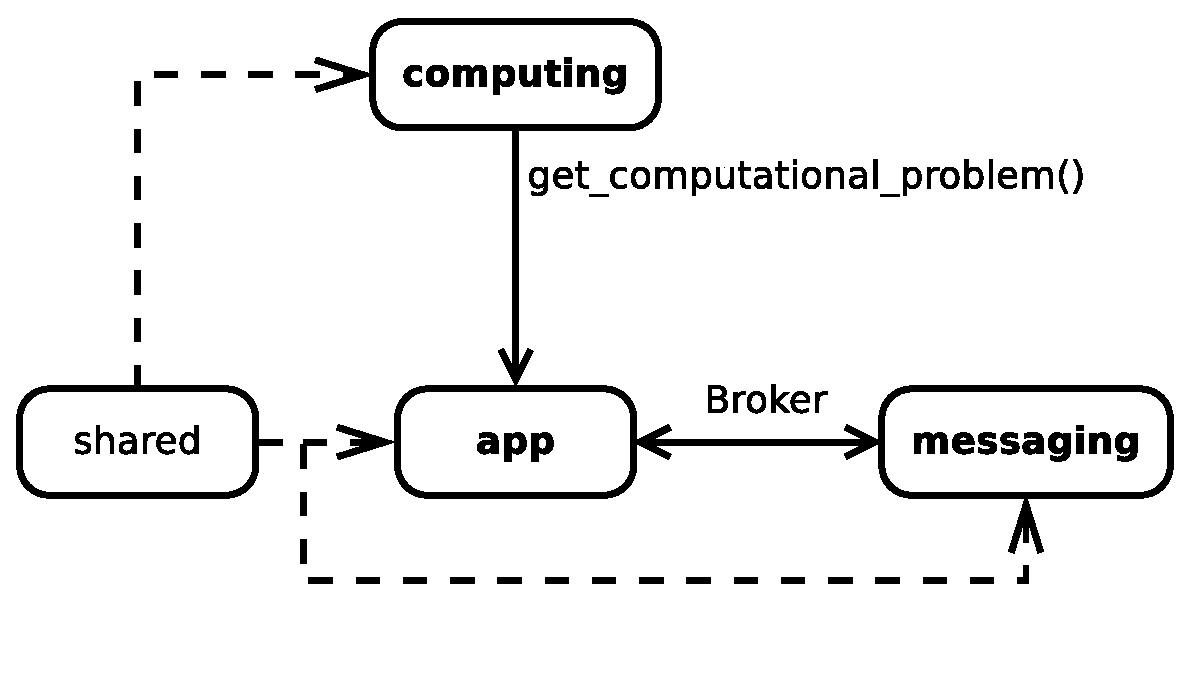
\includegraphics[width=\linewidth]{../diagrams/ProjectStructure.eps}
	\caption{Project Structure Diagram}
\end{figure}

Packages:
\begin{itemize}
    \item \textbf{app:} top-level package. It is the main thread of an application, responsible for managing other threads. It manages subproblem execution and communicates with the Broker. 
    The app package does not deal with network details directly: high-level commands are used instead of network packets.
    \item \textbf{messaging:} contains a Broker definition, an abstraction layer between the app and the computer network. 
    The Broker runs on a separate thread and listens to incoming packets, as well as sends commands received from the app package.
    \item \textbf{computing:} contains implementation details of computational problem.
    \item \textbf{shared:} contains utilities which are either used by all other packages, or are not unique to our project. 
    For instance, NetworkConnection (a socket wrapper class) could be easily used in other projects that utilise communication over network.
    \item \textbf{tests:} contains unit and integration tests that cover the rest of packages.
\end{itemize}

\section{Design patterns}
\subsection{Command}
\begin{figure}[H]
	\centering
	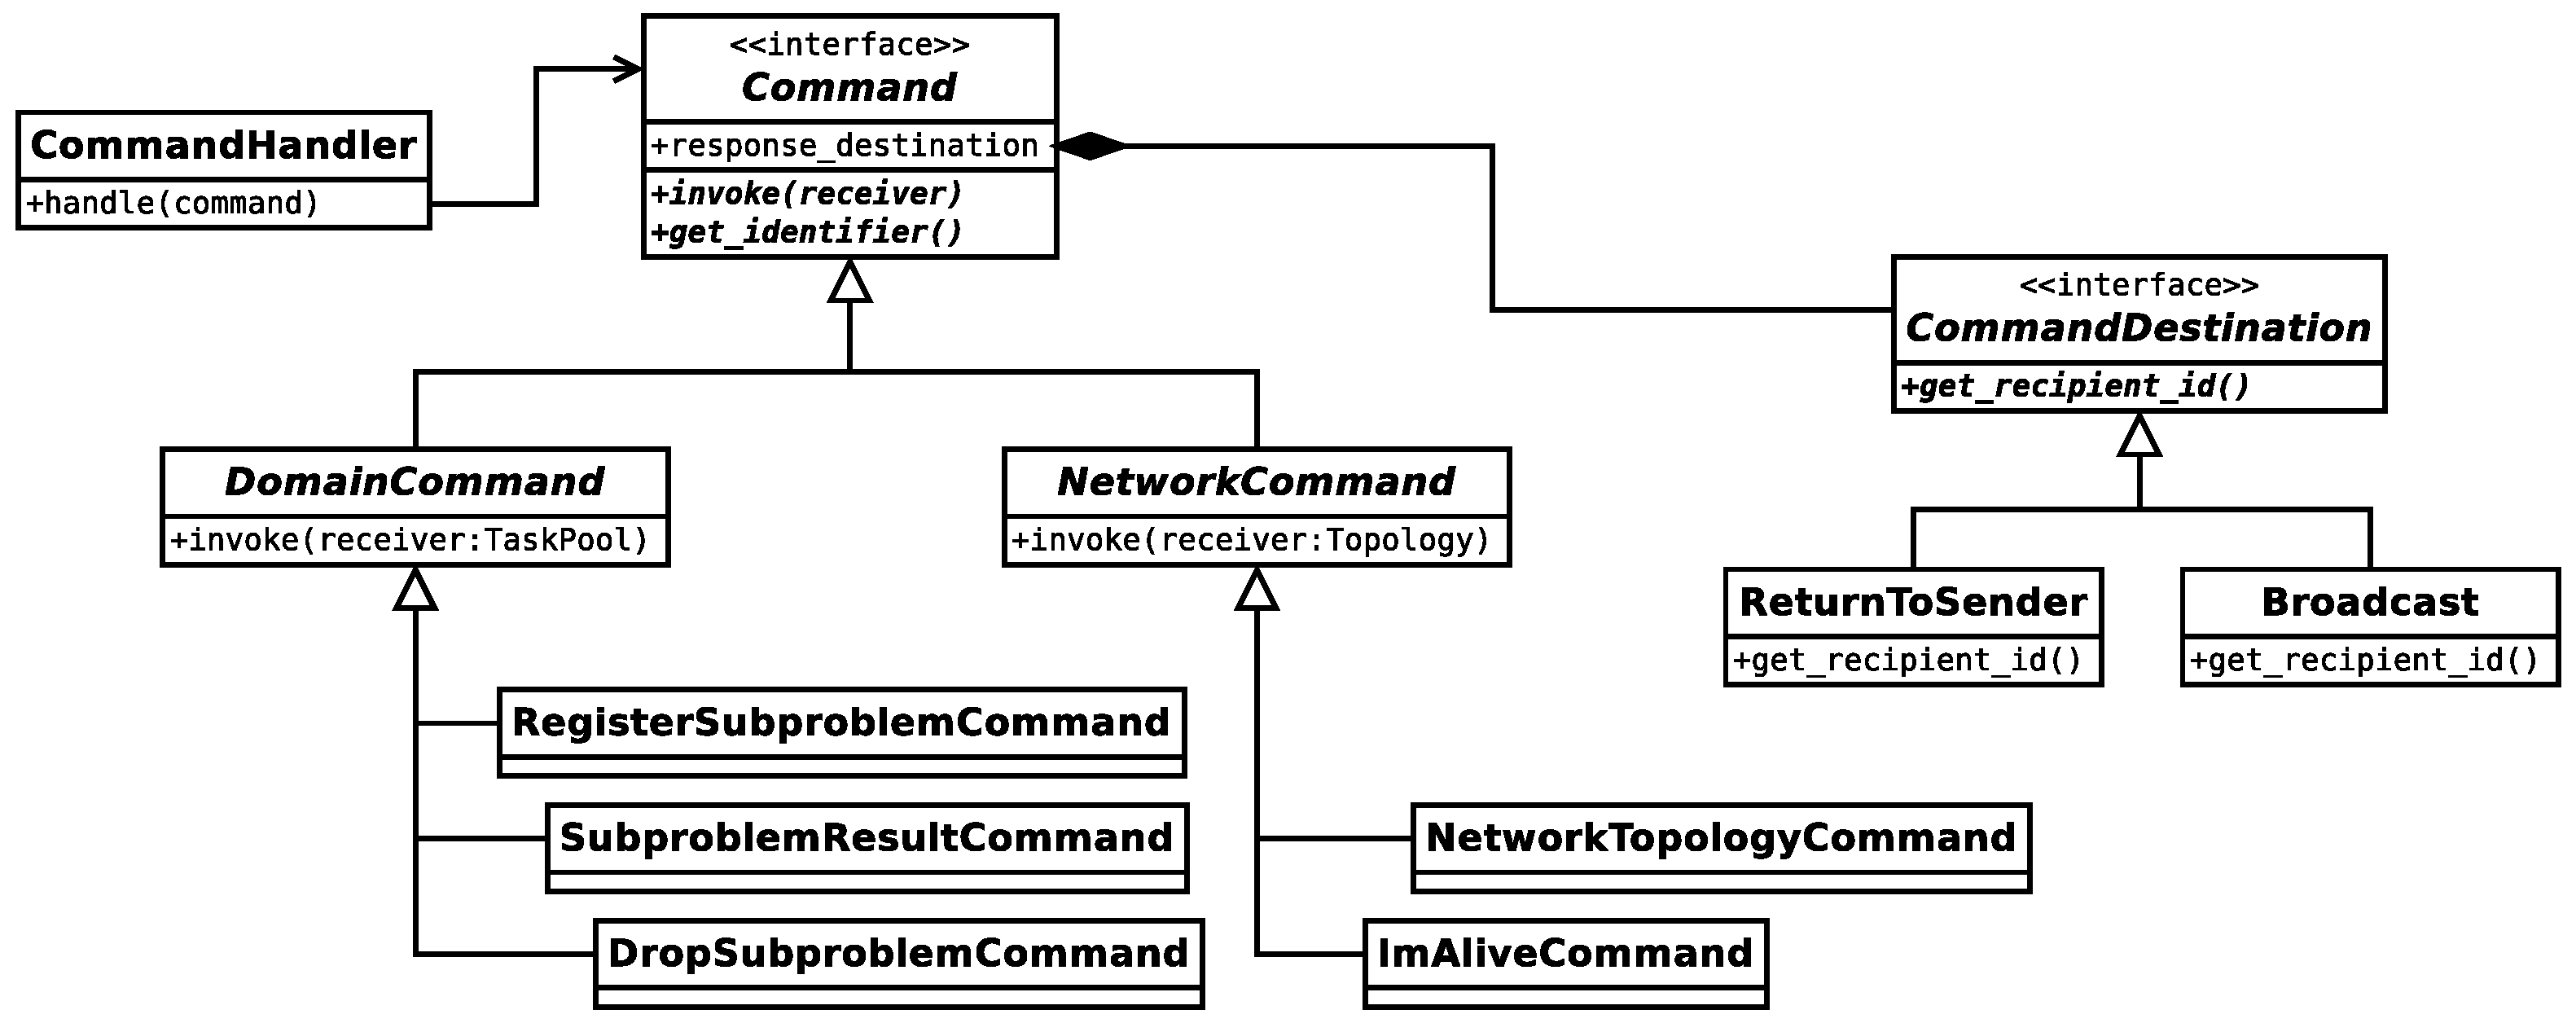
\includegraphics[width=\linewidth]{../diagrams/CommandDiagram.eps}
	\caption{Command Diagram}
\end{figure}

\subsection{Abstract Factory}
\begin{figure}[H]
	\centering
	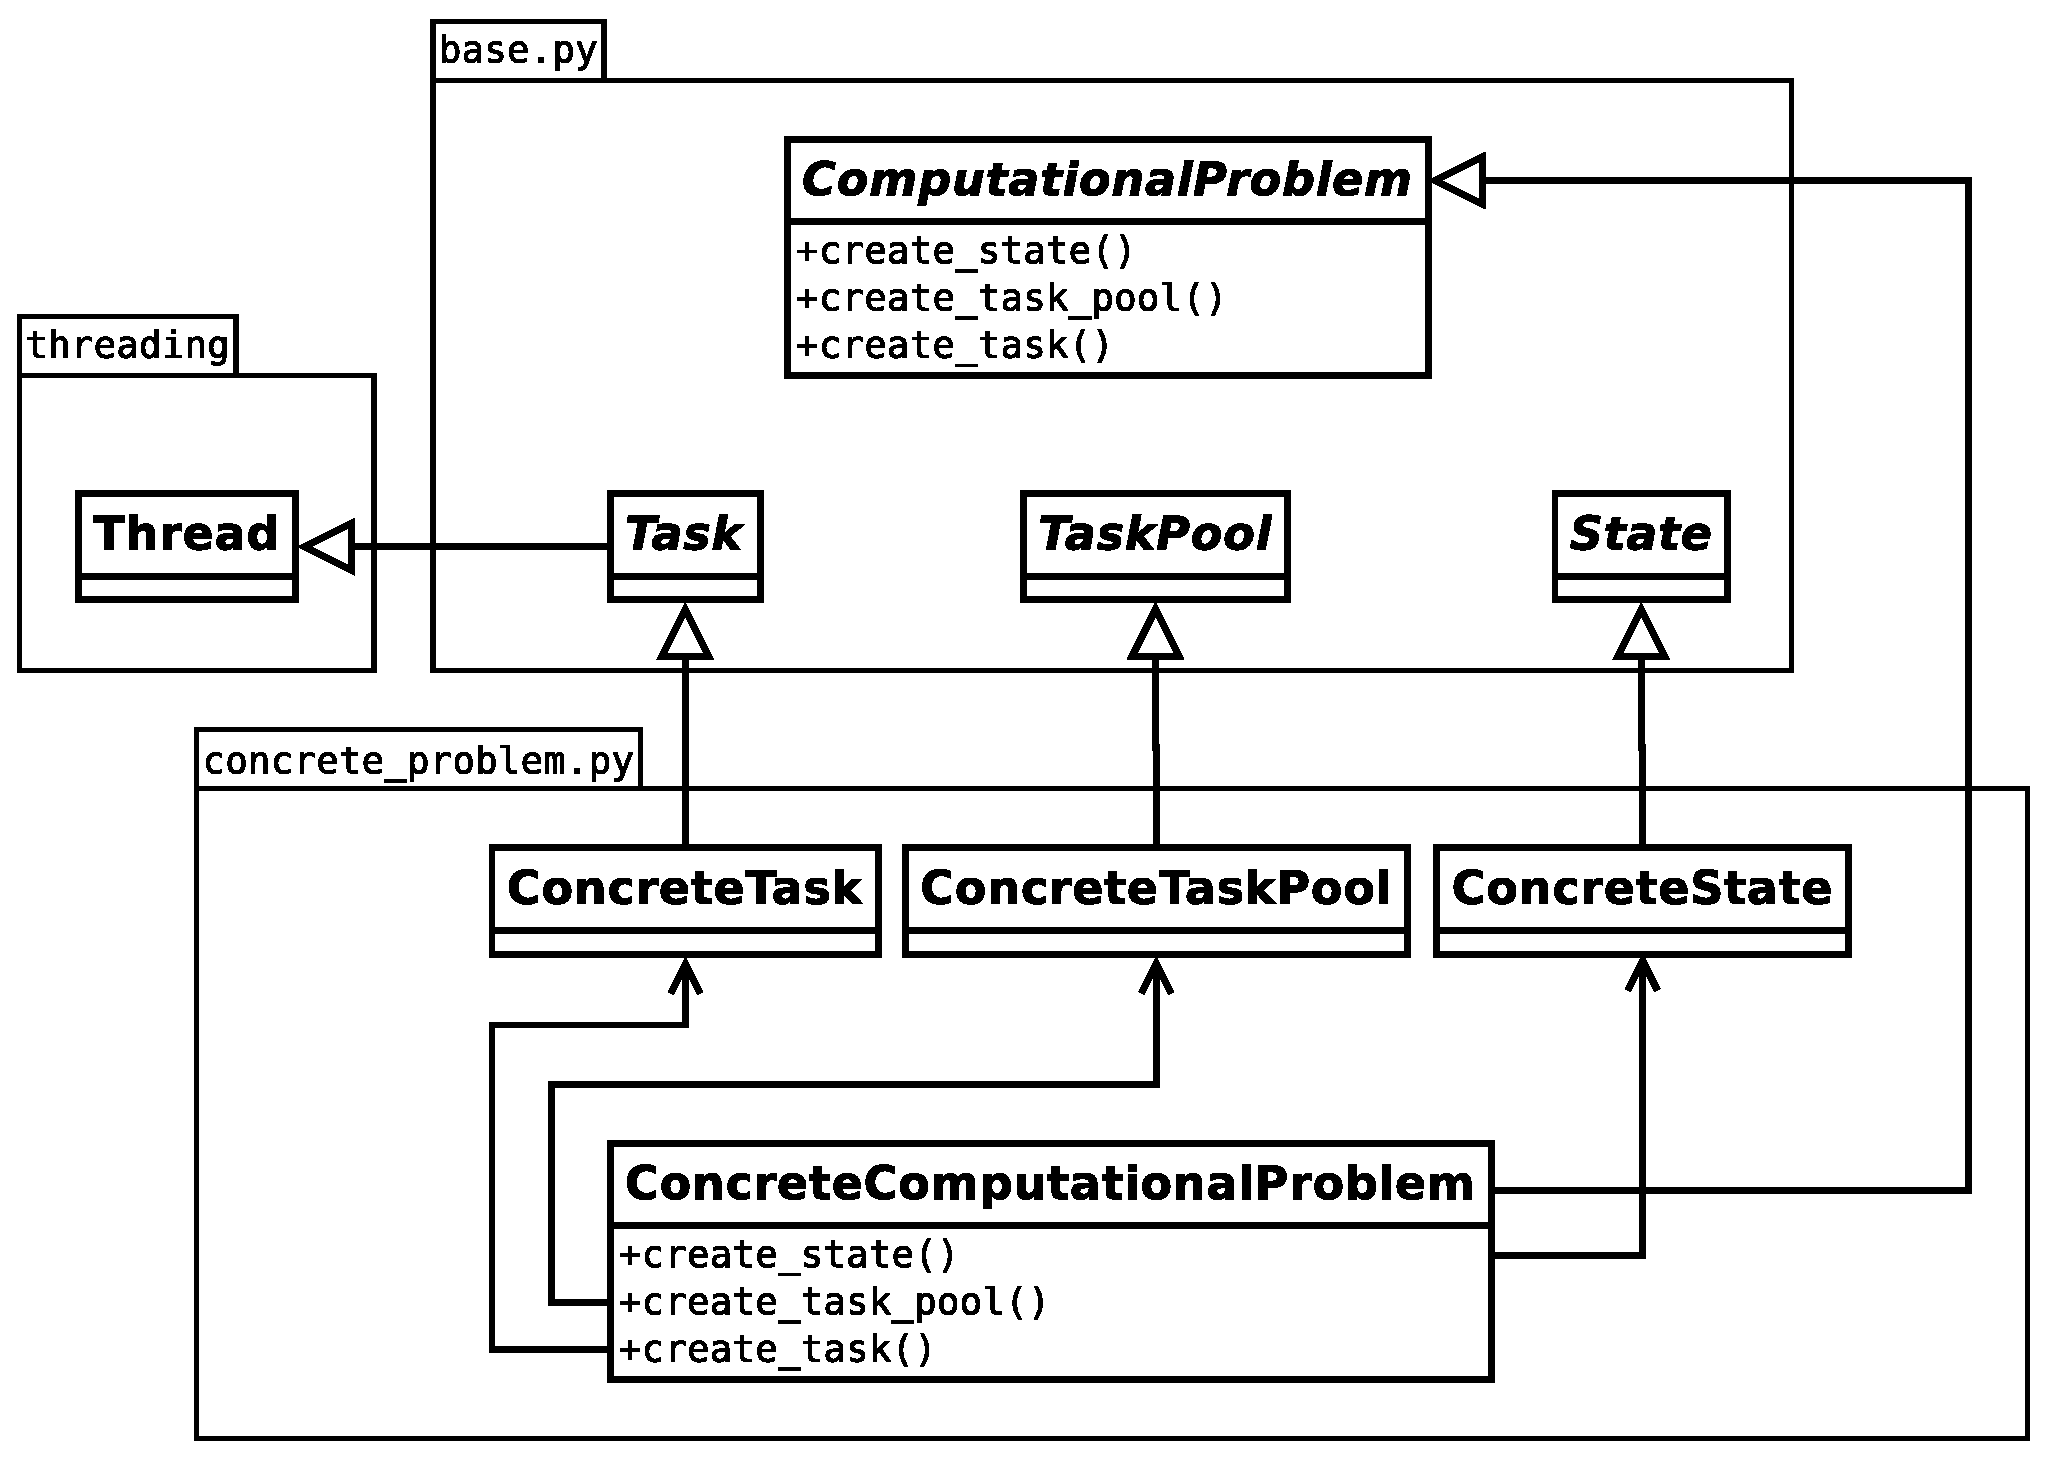
\includegraphics[width=\linewidth]{../diagrams/FactoryDiagram.eps}
	\caption{Computational Problem Abstract Factory Diagram}
\end{figure}

\subsection{Template Method}
\begin{figure}[H]
	\centering
	 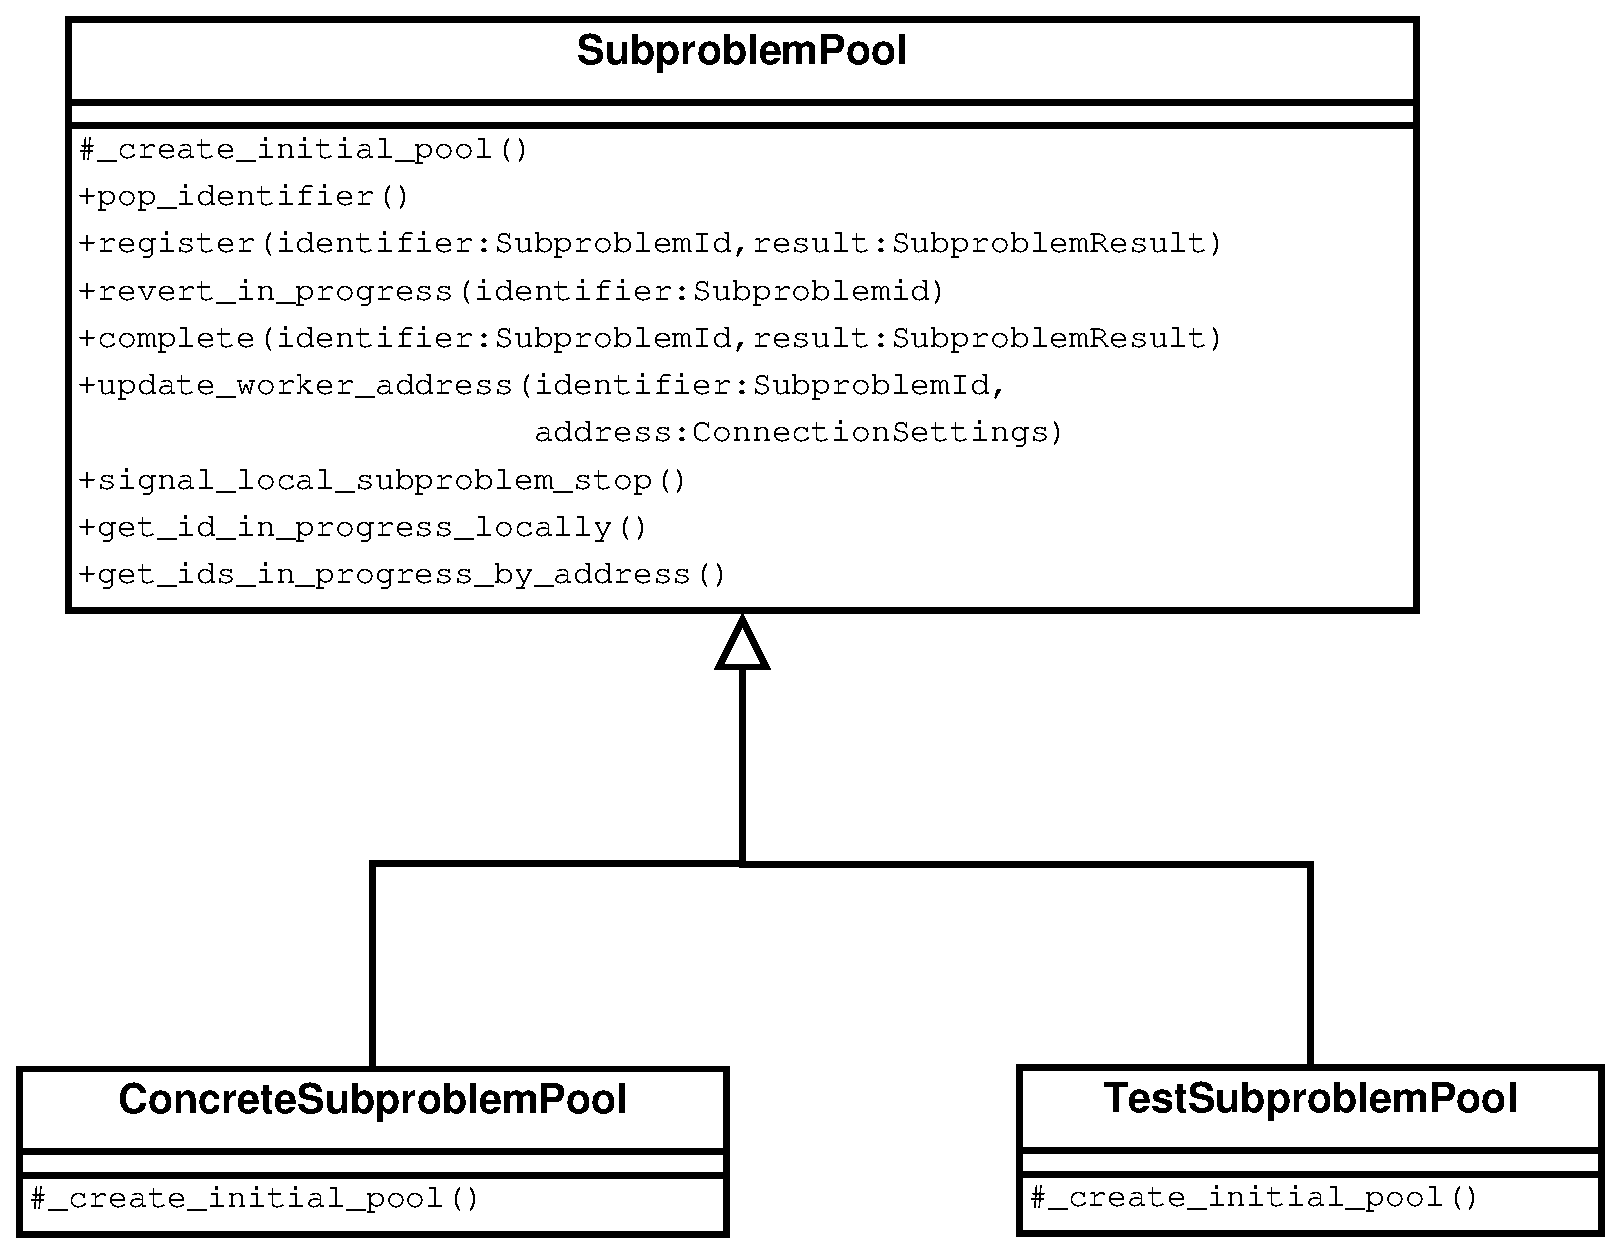
\includegraphics[width=.6\linewidth]{../diagrams/SubproblemPoolDiagram.eps}
	\caption{SubproblemPool Diagram}
\end{figure}

\subsection{Value Object}
Instead of~working with concrete types such as~strings or integers, we~often utilize so-called Value Objects (e.g. \texttt{SubproblemId}, \texttt{SubproblemResult}, \texttt{ConnectionSettings}). Thanks to~the \texttt{dataclass} decorator, instances of~these classes are immutable, and an auto-generated equality operator compares values rather than identities.

\section{Diagrams}
\begin{figure}[H]
	\centering
	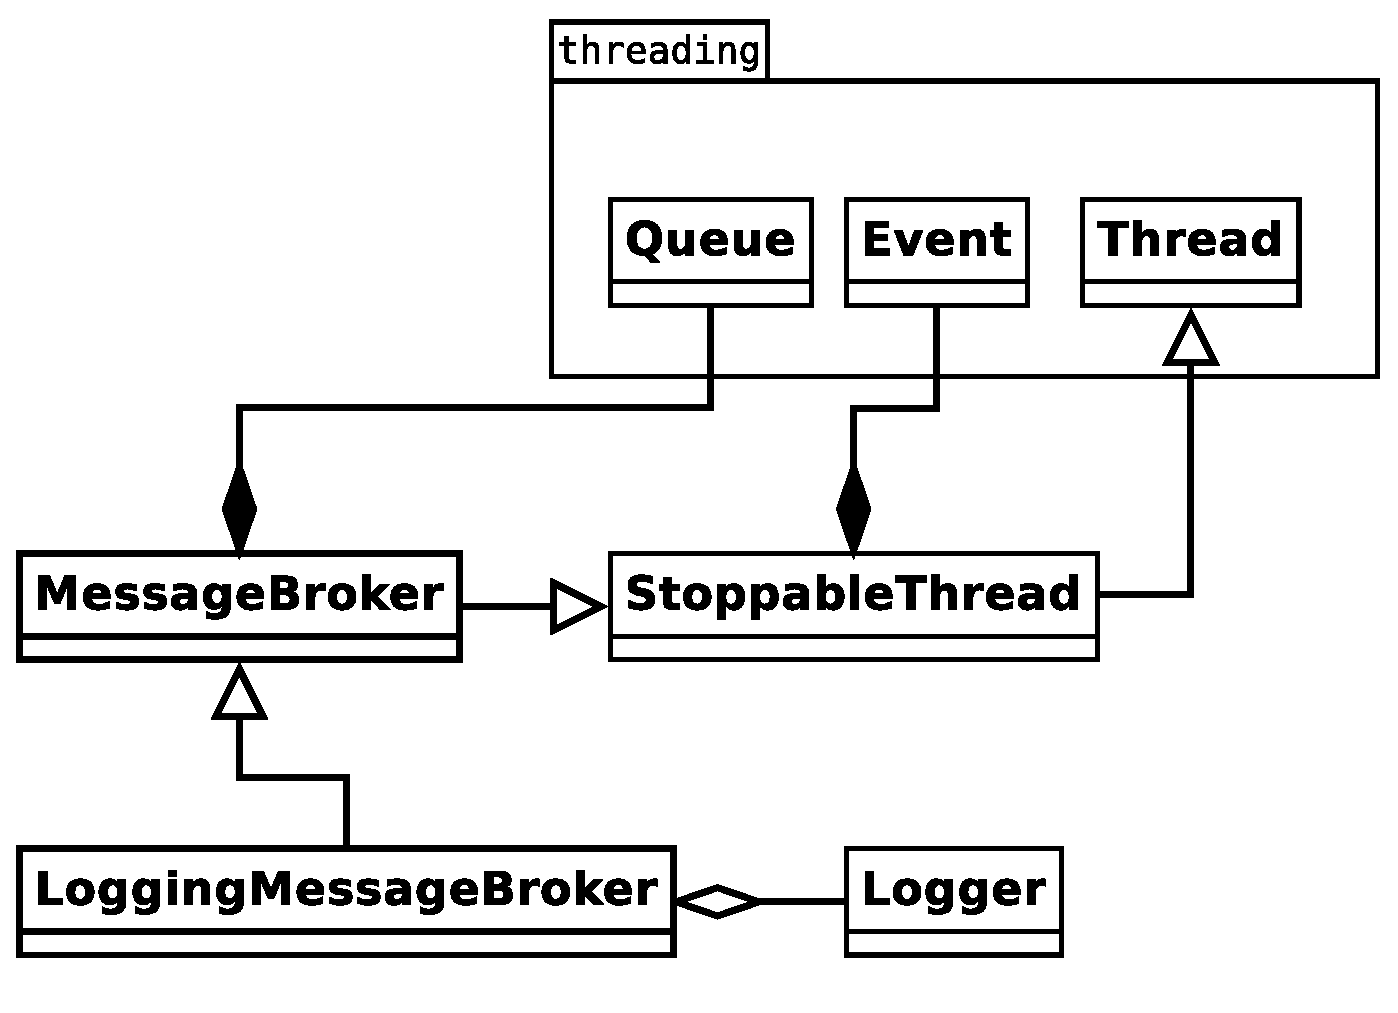
\includegraphics[width=\linewidth]{../diagrams/BrokerDiagram.eps}
	\caption{Broker Class Diagram}
\end{figure}

\begin{figure}[H]
	\centering
	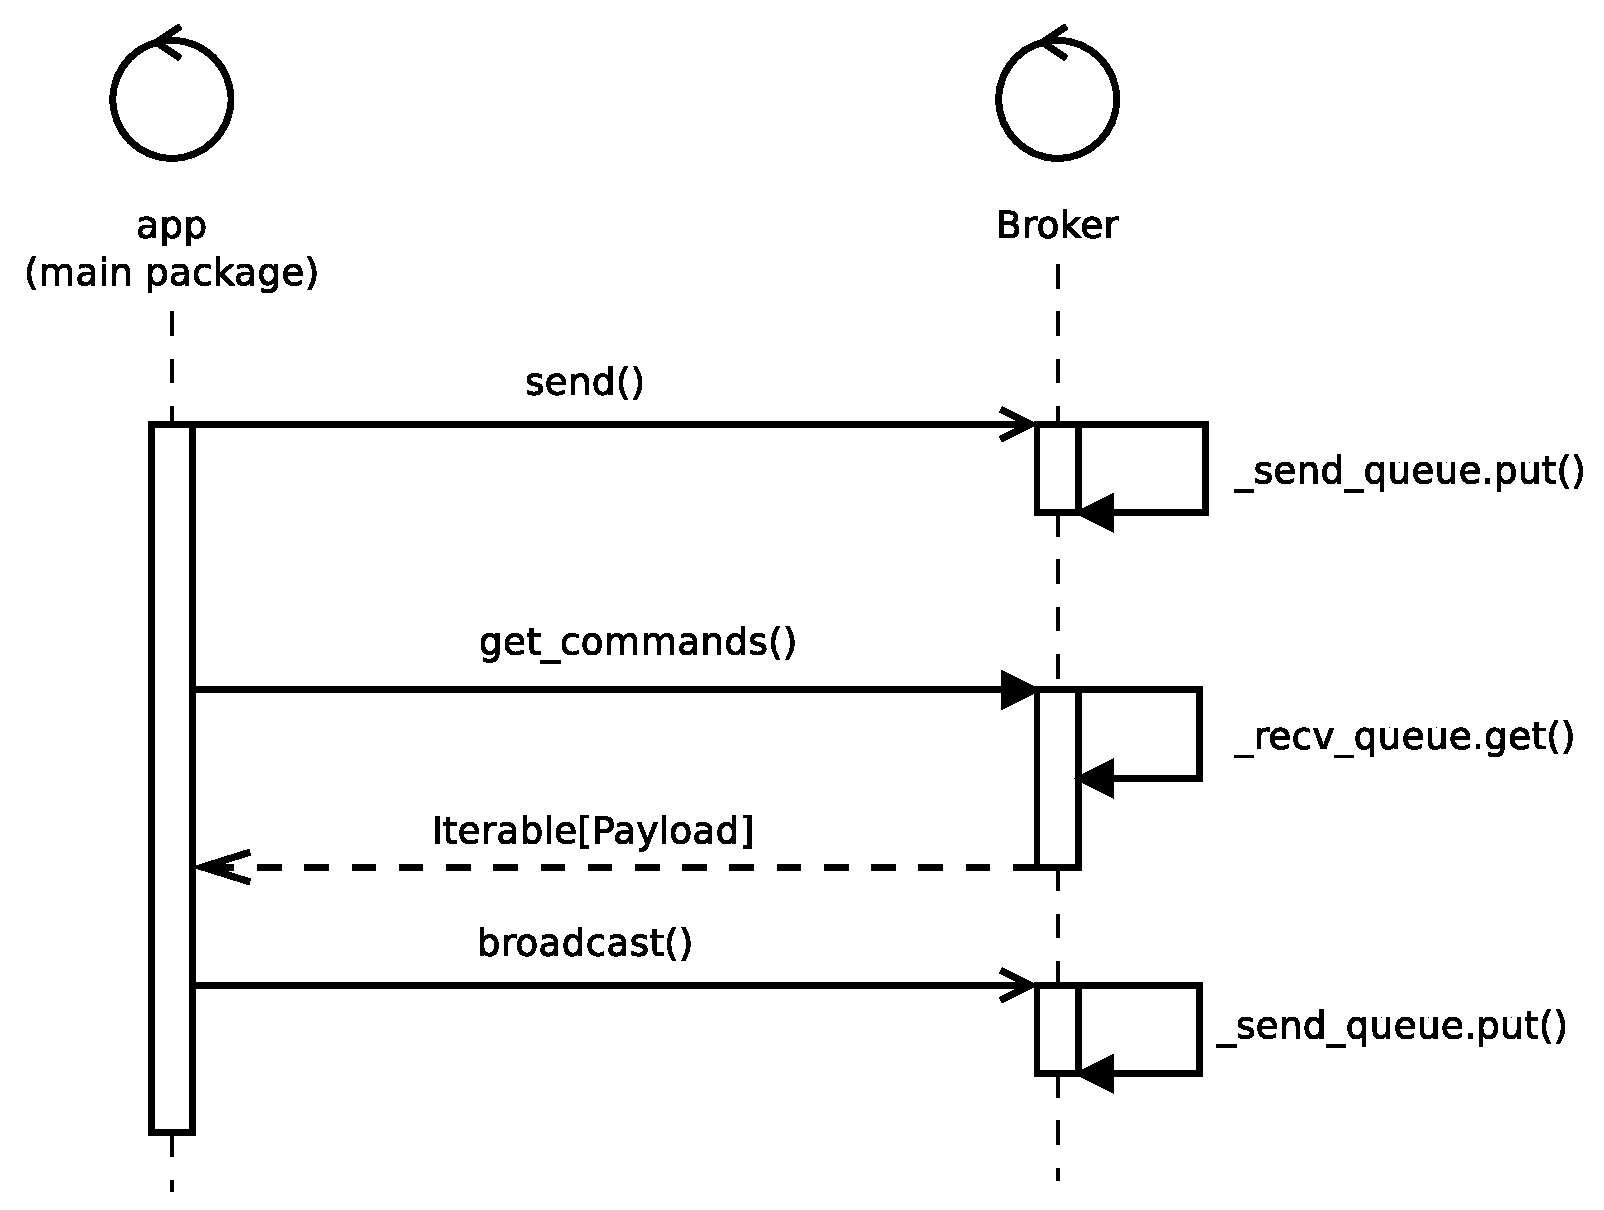
\includegraphics[width=\linewidth]{../diagrams/AppBrokerSequenceDiagram.eps}
	\caption{App-Broker Sequence Diagram}
\end{figure}

\newpage

\section{Security}
The possibilities to disrupt a computational network are plentiful:
\begin{itemize}
    \item “Flood” the network with fake result packets
    \item Deny all “register subproblem” requests
    \item Solve subproblems using a “malformed” state (e.g. replacing an original texture while rendering an image)
    \begin{itemize}
        \item Exchanging a state hash/control sum would help detect accidental mistakes. Malicious changes could be caught by solving a certain subproblem 
        several times (which still wouldn’t help if an attacker had control over nearly 50% of the network)
    \end{itemize}
    \item Disruption of data stored locally, in a file
    \begin{itemize}
        \item Little can we do to protect data against someone with a physical access to a machine
    \end{itemize}
    \item One computational network per actual computer network
    \begin{itemize}
        \item Introducing a kind of a session key might resolve the issue
    \end{itemize}
    \item Communication between agents is unencrypted
    \begin{itemize}
        \item Encryption itself will be easy to implement, if needed. It may be based on the aforementioned session key.
    \end{itemize}
\end{itemize}

\section{Technology}
\begin{itemize}
    \item \textbf{Python 3.7:} Python version 3.7. introduced @dataclass, which makes it easier to work with data structures.
    It allows creating immutable data structures.
    \item \textbf{Network Communication:} transmission of data in JSON format, using UDP protocol.
\end{itemize}

\end{document}